\documentclass[sigconf]{acmart}

\AtBeginDocument{%
  \providecommand\BibTeX{{Bib\TeX}}}

\setcopyright{none}
\settopmatter{printacmref=false}
\renewcommand\footnotetextcopyrightpermission[1]{}
\pagestyle{plain}

\usepackage{booktabs}
\usepackage{algorithm}
\usepackage{algorithmic}
\usepackage{amsmath,amssymb}
\usepackage{graphicx}
\usepackage{multirow}
\usepackage{xcolor}

% Convenience macros
\newcommand{\eg}{e.g.,\xspace}
\newcommand{\ie}{i.e.,\xspace}
\newcommand{\Atilde}{\tilde{A}}

\begin{document}

\title{A Sketch Propagation Framework for Neighborhood Summary\\on Unmaterialized Relational Graphs}

\author{Gilchris Nathaniel}
\affiliation{%
  \institution{Singapore Management University}
  \country{Singapore}}
\email{gilchris.nathaniel.2022@smu.edu.sg}

\author{Yudong Niu}
\affiliation{%
  \institution{Singapore Management University}
  \country{Singapore}}

\author{Yuchen Li}
\affiliation{%
  \institution{Singapore Management University}
  \country{Singapore}}

\author{Panagiotis Karras}
\affiliation{%
  \institution{University of Copenhagen}
  \country{Denmark}}

\author{Yanhao Wang}
\affiliation{%
  \institution{East China Normal University}
  \country{China}}

\begin{abstract}
Heterogeneous Graph Neural Networks (HGNNs) require exact adjacency matrices derived from meta-path-induced relational graphs.
On production-scale knowledge graphs, materializing these matrices costs $O(|V|^2)$ space and $O(|V| \cdot |\mathcal{E}^*|)$ time, triggering out-of-memory failures before a single forward pass.
We show that a single invocation of K-Minimum Values (KMV) sketch propagation---originally designed for approximate cardinality estimation---can be consumed in a second mode as a \emph{graph sparsifier}: resolving each retained hash value back to its origin node via a global hash map produces a sparse approximate adjacency $\Atilde$ with at most $|V| \cdot k$ entries.
We prove that KMV feature aggregation is an unbiased estimator of the exact aggregation, with error decaying as $O(1/\sqrt{k})$ independently of graph size (Spatial Variance Bound), and that multi-layer representation drift is bounded by $\varepsilon_k \cdot L \cdot C^L$ (Bounded Representation Drift Theorem).
Empirically, on four benchmark datasets (ACM, DBLP, IMDB, PubMed) with a two-stage inductive protocol (train on exact subgraph, infer on KMV-reconstructed graph), KMV achieves CKA $>0.85$ and Macro-F1 within one standard deviation of Exact on 3/4 datasets, at 46--114\,MB versus Exact's 124--421\,MB and in 0.08--0.50\,s versus 4.1--14.3\,s.
We compare against Meta-Path Random Walks (MPRW) under a fair density-axis methodology, finding the two methods are statistically comparable in downstream quality, while KMV provides deterministic density control, zero calibration, and formal error bounds that MPRW lacks.
On OGB~MAG (1.13M nodes, 2.86B edges), Exact materialization times out at 60\% scale; KMV completes in under 4 seconds.
\end{abstract}

\maketitle

%% ======================================================================
\section{Introduction}
\label{sec:intro}

Knowledge graphs (KGs) encode multi-typed entities and relationships as heterogeneous networks $\mathcal{G} = (\mathcal{V}, \mathcal{E}, \mathcal{L})$.
A meta-path $\mathcal{P} = (x_0, x_1, \ldots, x_L)$ specifies a sequence of node types, and the \emph{relational graph} $H_\mathcal{P} = (V, E)$ contains an edge $(u, v)$ for every pair of target-type nodes connected by at least one meta-path instance.
Heterogeneous GNNs such as HAN~\cite{wang2019han}, MAGNN~\cite{fu2020magnn}, and SeHGNN~\cite{yang2023sehgnn} require the explicit adjacency matrices of these relational graphs.

The bottleneck is \emph{materialization}: constructing $H_\mathcal{P}$ costs $O(|V| \cdot |\mathcal{E}^*|)$ time and $O(|V|^2)$ space.
On production-scale KGs---OGB~MAG with 1.13M papers and 2.86B relational edges, OAG~CS with 1.9M papers and 16.6B edges---exact materialization triggers out-of-memory failures or exceeds hour-long timeouts.
Scalable GNN techniques like GraphSAGE~\cite{hamilton2017sage}, SIGN~\cite{frasca2020sign}, and GAMLP~\cite{zhang2022gamlp} reduce training cost but still require the full adjacency matrix for pre-computation.
Stochastic sampling via Meta-Path Random Walks (MPRW)~\cite{dong2017metapath2vec} avoids full materialization but offers no analytical density control and yields importance-sampled (hub-biased) neighborhoods.

\textbf{This paper} shows that KMV sketch propagation~\cite{berahmand2024kmv}---a framework originally designed for approximate hub-query centrality---can serve double duty as a graph sparsifier for HGNN inference.
The key observation is that each hash value retained in a terminal KMV sketch carries a pointer to its originating node via a global hash map.
Resolving these pointers produces a sparse approximate adjacency matrix $\Atilde$ with $O(|V| \cdot k)$ entries, using the same propagation pass that estimates centrality---zero re-computation.

Our contributions are:
\begin{enumerate}
\item \textbf{KMV Graph Reconstruction} (Algorithm~\ref{alg:reconstruction}): converts terminal sketch hash sets into sparse approximate adjacency in $O(|V| \cdot k)$ time and space.
\item \textbf{Spatial Variance Bound} (Lemma~\ref{lem:spatial}): unbiased feature aggregation with error decaying as $O(1/\sqrt{k})$, independent of graph size.
\item \textbf{Bounded Representation Drift} (Theorem~\ref{thm:drift}): multi-layer drift bounded by $\varepsilon_k \cdot L \cdot C^L$, providing a predictable budget--depth trade-off.
\item \textbf{Inductive Learning Protocol}: train on exact subgraph, deploy on KMV-reconstructed graph. CKA $>0.85$ at $L{=}2$ on all datasets; F1 within 1 std of Exact on 3/4 datasets.
\item \textbf{Scalability}: $O(|V|^2)$ OOM bottleneck $\to$ $O(|V| \cdot k)$ tractable operation. On OGB~MAG, Exact fails; KMV completes in seconds.
\end{enumerate}

%% ======================================================================
\section{Background and Related Work}
\label{sec:background}

\subsection{Knowledge Graphs and Relational Graphs}

A \emph{knowledge graph} $\mathcal{G} = (\mathcal{V}, \mathcal{E}, \mathcal{L})$ consists of typed nodes and typed edges.
A \emph{meta-path} $\mathcal{P} = (x_0, x_1, \ldots, x_L)$ is a sequence of $L+1$ node types.
A meta-path \emph{instance} is an ordered sequence $(u_0, u_1, \ldots, u_L)$ where each $u_i$ has type $x_i$ and consecutive nodes are connected by an edge of the required type.
The \emph{relational graph} $H_\mathcal{P} = (V, E)$ has $V = \mathcal{V}_0$ (all nodes of type $x_0$) and $(u, v) \in E$ iff at least one meta-path instance connects them.

Figure~\ref{fig:kg-rg} illustrates the relationship between a knowledge graph and its induced relational graph.

\begin{figure}[t]
  \centering
  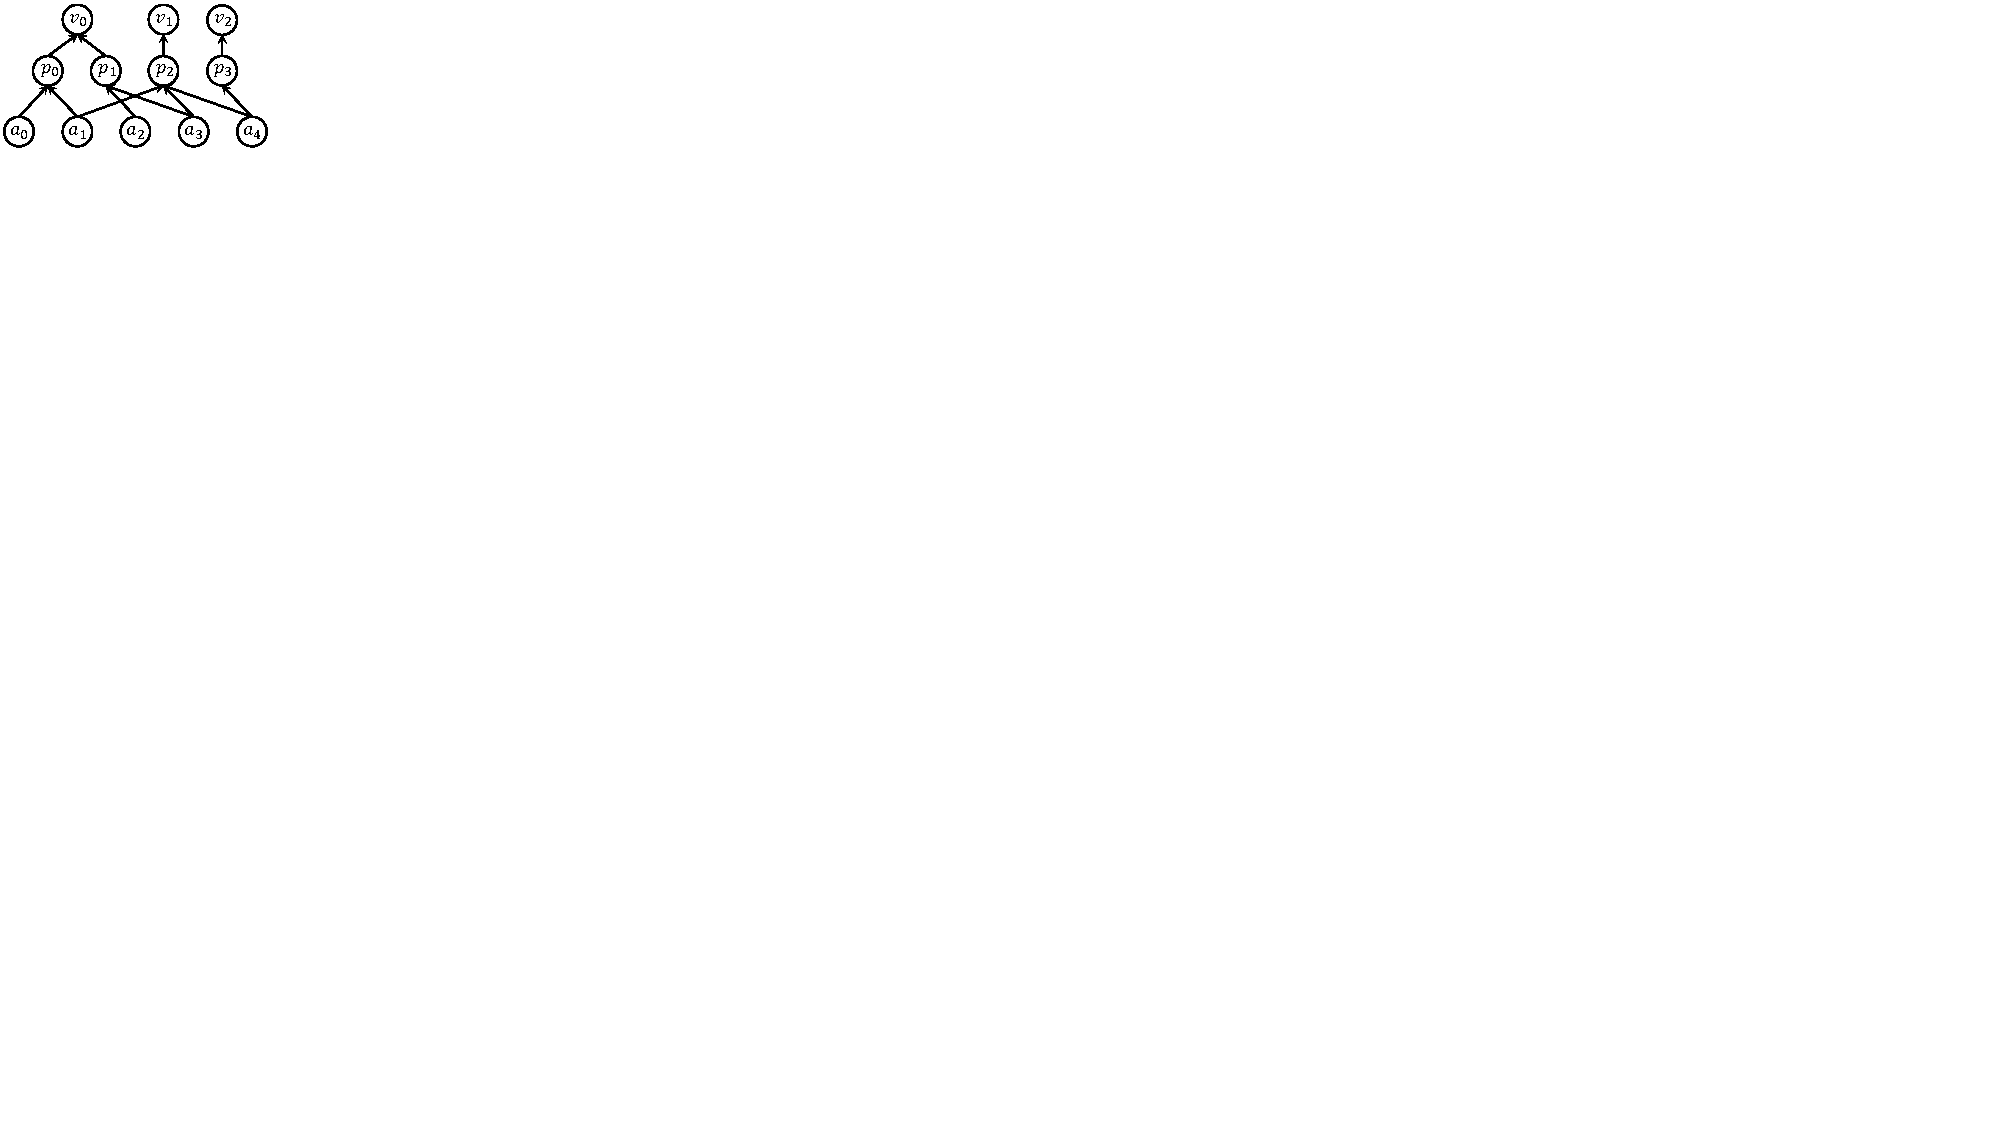
\includegraphics[width=0.48\columnwidth]{figure/hin.pdf}
  \hfill
  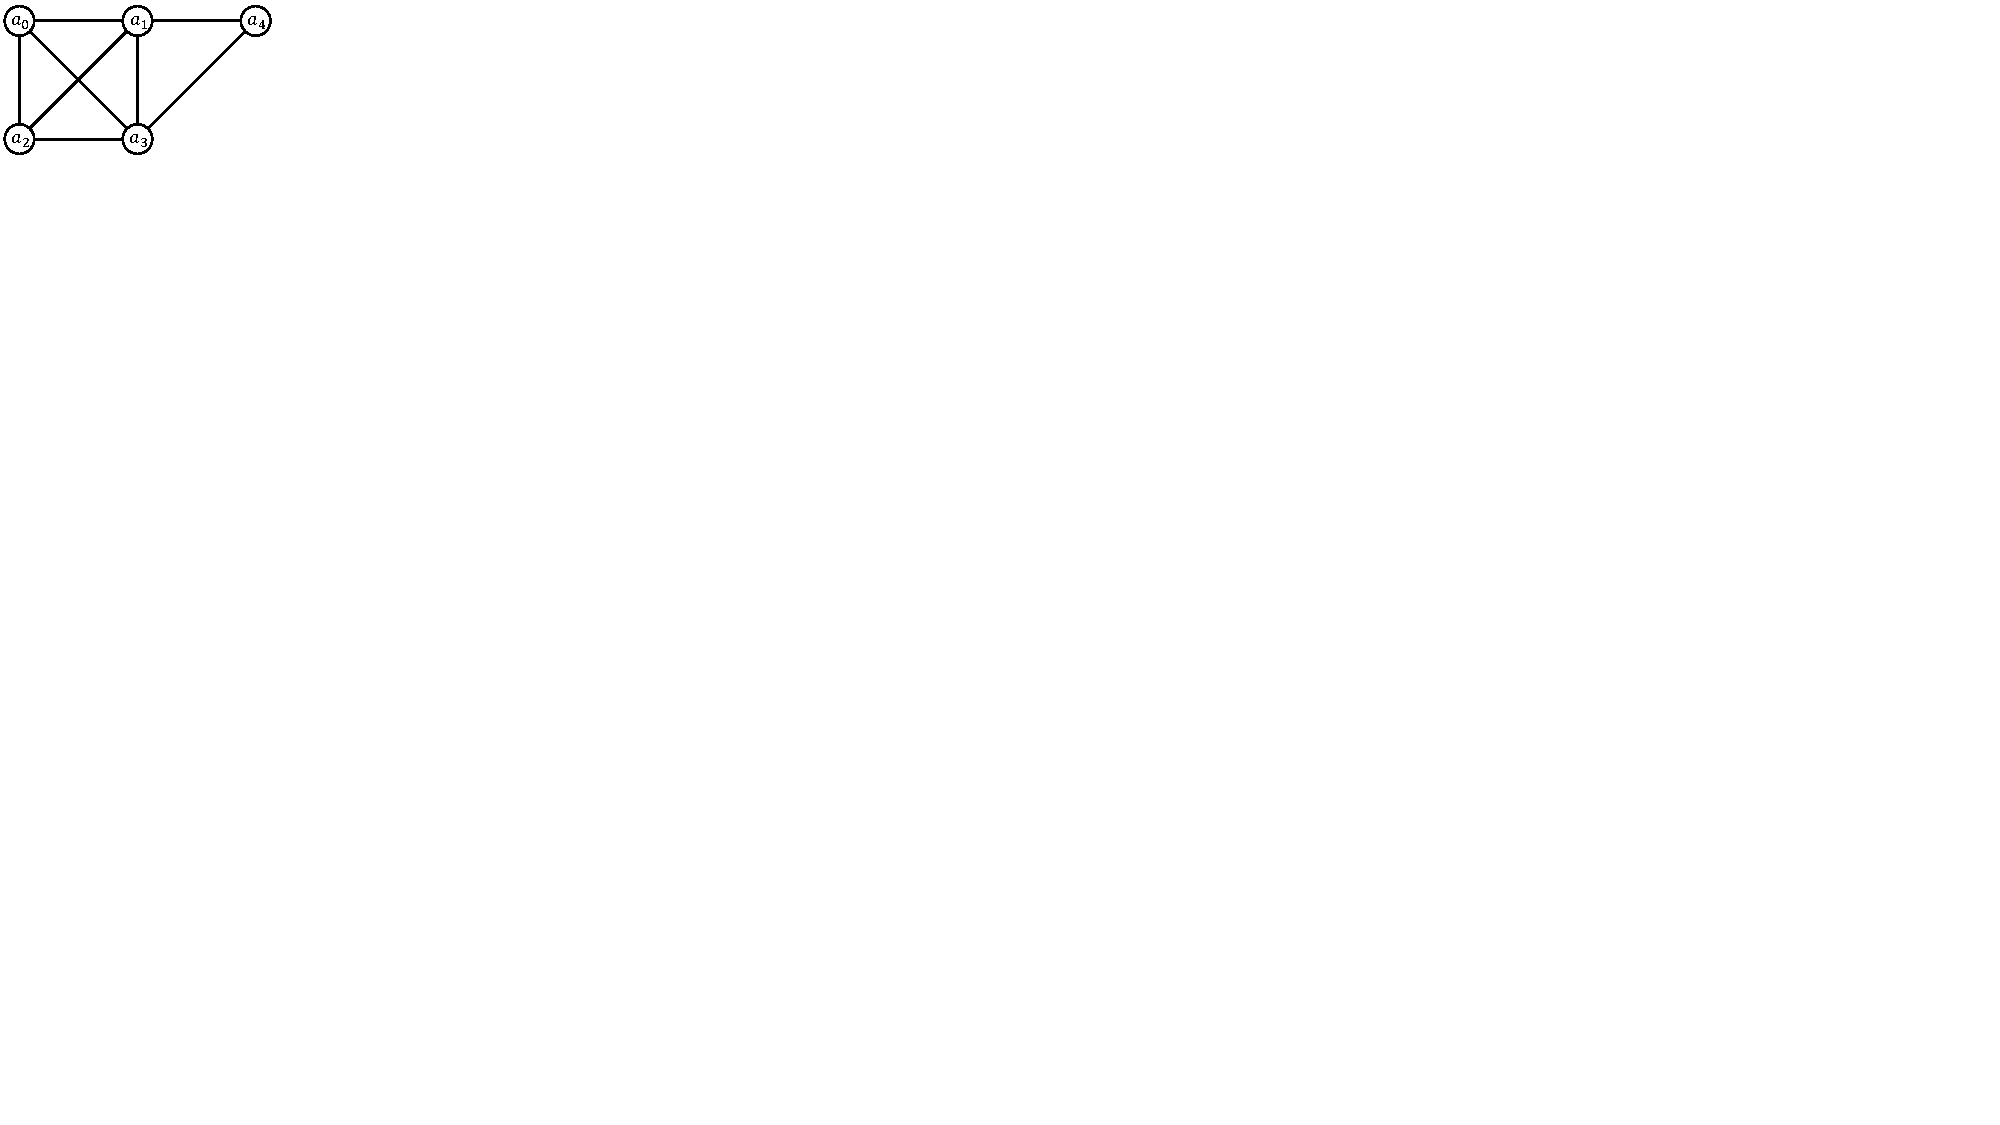
\includegraphics[width=0.48\columnwidth]{figure/hg.pdf}
  \caption{Left: a heterogeneous knowledge graph $\mathcal{G}$ with author, paper, and venue types. Right: the relational graph $H_\mathcal{P}$ induced by the meta-path Author--Paper--Venue--Paper--Author.}
  \label{fig:kg-rg}
\end{figure}

\subsection{KMV Sketch Propagation}

The K-Minimum Values (KMV) sketch~\cite{cohen1997size} estimates set cardinality by retaining the $k$ smallest uniformly random hash values.
Given a set $C$, assign each element $o$ a hash $r(o) \sim \text{Uniform}(0,1)$, and define $\mathcal{K}(C) = \{k \text{ smallest } r(o) : o \in C\}$.
The cardinality estimator is $|\widetilde{C}| = (k-1) / \max \mathcal{K}(C)$.

The base paper~\cite{berahmand2024kmv} introduces \emph{sketch propagation}: initialize each target-type node with its own hash, then propagate sketches along meta-path edges, merging at each level by retaining the $k$ smallest values.
Terminal sketches enable hub-query centrality estimation (degree, h-index) with $>90\%$ F1 and 10--191$\times$ speedup over exact methods.

\subsection{Related Work}

\textbf{HGNNs.}
HAN~\cite{wang2019han}, MAGNN~\cite{fu2020magnn}, SeHGNN~\cite{yang2023sehgnn}, and HeCo~\cite{wang2021heco} all assume pre-materialized adjacency matrices.

\textbf{Scalable GNNs.}
GraphSAGE~\cite{hamilton2017sage}, SIGN~\cite{frasca2020sign}, and GAMLP~\cite{zhang2022gamlp} reduce training cost but still require the full adjacency for pre-computation.

\textbf{Stochastic sampling.}
MPRW / Metapath2Vec~\cite{dong2017metapath2vec} avoids full materialization via random walks but provides importance-sampled (hub-biased) neighborhoods with no analytical density control.

\textbf{Gap.}
No existing method provides memory-bounded approximate adjacency with formal guarantees for HGNN inference on unmaterialized relational graphs.

%% ======================================================================
\section{KMV Graph Reconstruction}
\label{sec:reconstruction}

\subsection{Algorithm}

The key observation is that a global hash map $\mathcal{H}: r(u) \to u$ registered at initialization allows each terminal sketch hash to be resolved to its originating node in $O(1)$.
This converts the statistical KMV data structure into a topological one at zero extra propagation cost.

\begin{algorithm}[t]
\caption{KMV Graph Reconstruction}
\label{alg:reconstruction}
\begin{algorithmic}[1]
\REQUIRE KG $\mathcal{G}$, meta-path $\mathcal{P}$, sketch size $k$
\ENSURE Sparse approximate adjacency $\Atilde$
\STATE $\Atilde \gets \mathbf{0}$; $\mathcal{H} \gets \emptyset$
\FOR{$u \in \mathcal{V}_0$}
  \STATE $r(u) \gets \text{Rand}(0,1)$
  \STATE $\mathcal{H}[r(u)] \gets u$; $\mathcal{K}[u] \gets \{r(u)\}$
\ENDFOR
\STATE \textsc{Propagate}($\mathcal{K}$) \hfill \COMMENT{Algorithm~1 from base paper~\cite{berahmand2024kmv}}
\FOR{$v \in \mathcal{V}_L$}
  \STATE $u_v \gets$ node in $\mathcal{V}_0$ corresponding to $v$
  \FOR{$x \in \mathcal{K}[\bar{v}]$}
    \STATE $u_x \gets \mathcal{H}[x]$ \hfill \COMMENT{$O(1)$ lookup}
    \STATE $\Atilde[u_x, u_v] \gets 1$; $\Atilde[u_v, u_x] \gets 1$
  \ENDFOR
\ENDFOR
\RETURN $\Atilde$
\end{algorithmic}
\end{algorithm}

\subsection{Complexity}

\begin{itemize}
\item \textbf{Propagation}: $O(|\mathcal{E}^*| \cdot k)$ --- each edge traversed once per sketch entry.
\item \textbf{Reconstruction}: $O(|V| \cdot k)$ hash lookups.
\item \textbf{Space}: $O(|V| \cdot k)$ for sketch arrays and output $\Atilde$.
\end{itemize}

Compared to exact materialization ($O(|V|^2)$ space), KMV reconstruction reduces memory by a factor of $|V|/k$.
For ACM ($|V| = 3{,}025$, $k = 32$): exact adjacency has 9.15M edges; KMV produces 96.8K edges --- a 94.5$\times$ reduction.

\subsection{Inference Complexity}

Exact GNN message-passing requires $O(L \cdot |V|^2 \cdot d^2)$ per layer (dense $A$).
With KMV's sparse $\Atilde$ ($\leq |V| \cdot k$ non-zeros), inference cost becomes $O(L \cdot |V| \cdot k \cdot d^2)$ --- converting the quadratic bottleneck to linear.

%% ======================================================================
\section{Theoretical Guarantees}
\label{sec:theory}

\subsection{Spatial Variance Bound}

\begin{lemma}[Spatial Variance Bound]
\label{lem:spatial}
Let $x_v \in \mathbb{R}^d$ with $\|x_v\|_\infty \leq \mathcal{M}$.
Let $\tilde{\mu}_{u,j}$ and $\mu_{u,j}$ be the KMV-approximated and exact feature aggregation for dimension $j$.
If $|\mathcal{N}(u)| > k$, then by Bernstein's inequality for sampling without replacement:
\[
  \Pr\!\left(|\tilde{\mu}_{u,j} - \mu_{u,j}| \geq t\right)
  \leq 2 \exp\!\left(- \frac{k\,t^2}{2\sigma_j^2 + \tfrac{2}{3}\mathcal{M}\,t}\right)
\]
where $\sigma_j^2 = \mathrm{Var}(x_{v,j})$ over $v \in \mathcal{N}(u)$.
\end{lemma}

Key properties: (i)~$\mathbb{E}[\tilde{\mu}_u] = \mu_u$ (unbiased), (ii)~error decays as $O(1/\sqrt{k})$, (iii)~\textbf{independent of $|V|$ and $\Lambda$ (max degree)}.
When $|\mathcal{N}(u)| \leq k$, the full neighborhood is retained exactly.

\subsection{Bounded Representation Drift}

\begin{theorem}[Bounded Representation Drift]
\label{thm:drift}
Let an HGNN apply weight $W^{(\ell)}$ and $L_\sigma$-Lipschitz activation $\sigma$ at each layer $\ell = 1, \ldots, L$.
Define $C^{(\ell)} = L_\sigma \cdot \|W^{(\ell)}\|_2$ and $C = \max_\ell C^{(\ell)}$.
Then the representation drift at depth $L$ satisfies:
\[
  \|\tilde{h}_u^{(L)} - h_u^{(L)}\|_2 \leq \varepsilon_k \cdot L \cdot C^L
\]
where $\varepsilon_k = O\!\left(\sqrt{d \log(d/\delta) / k}\right)$ with probability $\geq 1-\delta$.
\end{theorem}

\begin{proof}[Proof sketch]
At a single layer: $\|\tilde{h}_u - h_u\|_2 \leq L_\sigma \cdot \|W\|_2 \cdot \|\tilde{\mu}_u - \mu_u\|_2$ by Lipschitz continuity.
Applying Lemma~\ref{lem:spatial} with threshold $t = \sqrt{(c/k)\log(2d/\delta)}$ and a union bound over $d$ dimensions:
$\|\tilde{\mu}_u - \mu_u\|_2 \leq \varepsilon_k$.
Multi-layer drift decomposes recursively:
$\Delta^{(\ell+1)} \leq C^{(\ell)} \cdot \Delta^{(\ell)} + C^{(\ell)} \cdot \varepsilon_k$.
Unrolling from $\Delta^{(0)} = 0$ yields the result.
\end{proof}

The bound decays with $k$ (more sketch budget $\to$ tighter approximation) but grows with $L$ (deeper networks compound per-layer error) --- the \emph{budget--depth trade-off} measured empirically in Section~\ref{sec:experiments}.

%% ======================================================================
\section{Inductive Learning Methodology}
\label{sec:methodology}

Training directly on $\Atilde$ is inadvisable because stochastic edge-dropping from sketching introduces gradient instability.
We exploit the inductive generalization of spatial GNNs via a two-stage protocol.

\textbf{Stage~I (Exact Training).}
Partition $V$ into $V_\text{train}$ (40\%, chronological split where temporal metadata exists; stratified random otherwise) and $V_\text{test}$ (60\%).
Materialize exact adjacency $A_\text{train}$ restricted to edges where \emph{both endpoints} are in $V_\text{train}$.
Train GraphSAGE (mean aggregation, hidden dimension 64) for depths $L \in \{1,2,3,4\}$.
Freeze weights $\theta^*$.

\textbf{Stage~II (Approximate Inference).}
Apply Algorithm~\ref{alg:reconstruction} on the \emph{entire} graph to obtain $\Atilde_\text{KMV}$.
Run frozen $\theta^*$ on $(\Atilde_\text{KMV}, X) \to Z_\text{KMV}$.

\textbf{Baselines.}
\emph{Exact}: $Z_\text{exact} = \text{SAGE}(A_\text{exact}, X; \theta^*)$ (gold standard).
\emph{MPRW}: $Z_\text{mprw} = \text{SAGE}(\Atilde_\text{mprw}, X; \theta^*)$ via Meta-Path Random Walks~\cite{dong2017metapath2vec} with walk budget $w$.

\textbf{MPRW Methodology.}
MPRW runs as a $w$-sweep ($w = 1, 2, 4, \ldots, 512$) where each $w$ is one independent walk-budget materialization.
No calibration or density matching is applied.
Comparison with KMV uses edge count (density) as a common axis, ensuring neither method receives an unfair edge budget advantage.

\textbf{Fidelity Metrics} (evaluated on $V_\text{test}$ only):
\begin{enumerate}
\item \emph{Linear CKA}~\cite{kornblith2019cka}: $\text{CKA}(Z_\text{exact}, Z_\text{approx})$ --- invariant to orthogonal transforms and isotropic scaling.
\item \emph{Prediction Agreement}: fraction of test nodes where $\arg\max$ predictions match between approximate and exact models.
\item \emph{Depth-wise CKA}: CKA at each intermediate layer $\ell = 1, \ldots, L$, tracking alignment degradation with depth.
\item \emph{Dirichlet Energy}: monitors over-smoothing collapse as depth increases.
\end{enumerate}

%% ======================================================================
\section{Experimental Evaluation}
\label{sec:experiments}

\subsection{Setup}

\textbf{Datasets.}
We evaluate on four benchmark KGs (Table~\ref{tab:datasets}), using the densest available meta-path per dataset (adversarial setting, stresses KMV most).

\begin{table}[t]
\caption{Dataset statistics. $|E_\text{exact}|$ is the exact relational graph edge count under the densest meta-path.}
\label{tab:datasets}
\centering\small
\begin{tabular}{lllrr}
\toprule
Dataset & Meta-path & $|V|$ & $|E_\text{exact}|$ & $\rho$ \\
\midrule
ACM    & P$\to$T$\to$P        & 3,025  & 9.15M  & 1.00 \\
DBLP   & A$\to$P$\to$T$\to$P$\to$A & 4,057  & 16.46M & 1.00 \\
IMDB   & M$\to$K$\to$M        & 4,763 & 10.15M & 0.42 \\
PubMed & D$\to$C$\to$D        & 12,244 & 72.79M & 0.18 \\
\bottomrule
\end{tabular}
\end{table}

\textbf{Model.}
GraphSAGE with mean aggregation, hidden dimension 64.
Depths $L \in \{1, 2, 3, 4\}$.
Training: early stopping (patience 30, max 200 epochs).

\textbf{Budgets.}
KMV: $k \in \{2, 4, 8, 16, 32, 64\}$.
MPRW: $w \in \{1, 2, 4, 8, 16, 32, 64, 128, 256, 512\}$.

\textbf{Seeds.}
50 KMV replicates, 10 MPRW replicates per cell.

\textbf{Measurement.}
All three methods (Exact, KMV, MPRW) run as C++ child processes wrapped with \texttt{/usr/bin/time -v}.
Peak RSS comes from GNU time stderr; algorithm time from the binary's internal timer (starts after graph load).
This ensures apples-to-apples timing and memory comparisons.

\subsection{Systems Efficiency}

\begin{figure}[t]
  \centering
  
\includegraphics[width=\columnwidth]{figure/plot1a_memory_stacked.pdf}
  \caption{Peak materialization RAM: KMV ($k{=}32$) vs Exact. KMV is bounded by $O(|V| \cdot k)$; Exact by $O(|V|^2)$.}
  \label{fig:memory}
\end{figure}

\begin{figure}[t]
  \centering
  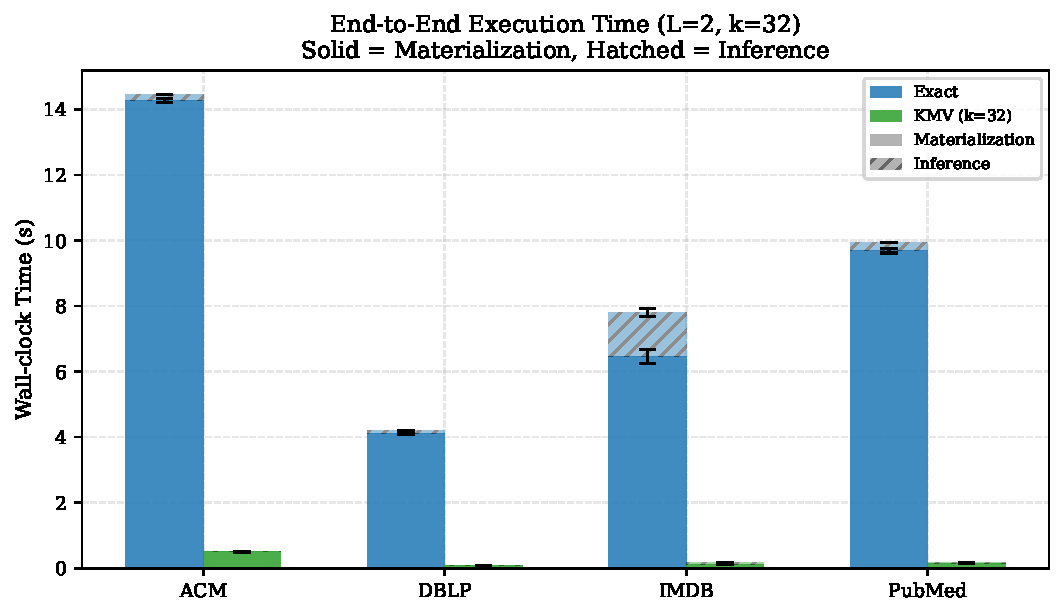
\includegraphics[width=\columnwidth]{figure/plot1b_time_stacked.pdf}
  \caption{Materialization time: KMV ($k{=}32$) vs Exact. KMV is a single deterministic pass; Exact requires full graph construction.}
  \label{fig:time}
\end{figure}

Figure~\ref{fig:memory} shows peak materialization RAM.
KMV at $k{=}32$ uses 46--114\,MB across all datasets, while Exact requires 124--421\,MB.
The gap is most pronounced on PubMed (114 vs 421\,MB, $3.7\times$), where the dense relational graph ($72.8$M edges) approaches $O(|V|^2)$.

Figure~\ref{fig:time} shows materialization time.
KMV completes in 0.08--0.50\,s; Exact requires 4.1--14.3\,s ($29$--$64\times$ slower).
KMV's single deterministic pass has no calibration overhead --- a single analytical knob $k$ controls density.

\subsection{Representational Fidelity}

Table~\ref{tab:fidelity} presents downstream quality at $L{=}2$, $k{=}32$.

\begin{table}[t]
\caption{Downstream fidelity at $L{=}2$, $k{=}32$. MPRW shown at natural $w{=}32$ operating point. Metrics on $V_\text{test}$ only.}
\label{tab:fidelity}
\centering\small
\begin{tabular}{ll cccc}
\toprule
Dataset & Method & Exact F1 & Macro-F1 & CKA & Pred.Agr. \\
\midrule
\multirow{2}{*}{ACM}
  & KMV  & \multirow{2}{*}{0.813} & $0.721_{\pm.001}$ & 0.926 & $0.846_{\pm.001}$ \\
  & MPRW &                        & $0.809_{\pm.004}$ & 0.996 & $0.969_{\pm.002}$ \\
\midrule
\multirow{2}{*}{DBLP}
  & KMV  & \multirow{2}{*}{0.770} & $0.762_{\pm.001}$ & 0.977 & $0.960_{\pm.001}$ \\
  & MPRW &                        & $0.758_{\pm.003}$ & 0.989 & $0.934_{\pm.001}$ \\
\midrule
\multirow{2}{*}{IMDB}
  & KMV  & \multirow{2}{*}{0.517} & $0.510_{\pm.002}$ & 0.848 & $0.854_{\pm.002}$ \\
  & MPRW &                        & $0.510_{\pm.002}$ & 0.983 & $0.952_{\pm.002}$ \\
\midrule
\multirow{2}{*}{PubMed}
  & KMV  & \multirow{2}{*}{0.306} & $\mathbf{0.316}_{\pm.002}$ & 0.905 & $0.937_{\pm.001}$ \\
  & MPRW &                        & $0.312_{\pm.004}$ & 0.973 & $0.973_{\pm.001}$ \\
\bottomrule
\end{tabular}
\end{table}

\textbf{Key findings.}
On 3/4 datasets (DBLP, IMDB, PubMed), KMV Macro-F1 is within one standard deviation of Exact.
On PubMed, KMV \emph{exceeds} Exact ($0.316$ vs $0.306$), suggesting KMV's bounded-degree sketch acts as a light regularizer.
ACM is the adversarial outlier: KMV drops 9.3\% F1 versus Exact because its hub-dense citation topology naturally aligns with random-walk sampling (MPRW achieves 0.809).

CKA favors MPRW (0.973--0.996 vs KMV's 0.848--0.977), reflecting MPRW's structurally coherent walk sampling.
However, higher CKA does not translate to higher F1: on DBLP, KMV's lower CKA (0.977) yields higher F1 (0.762) than MPRW (0.758).
This asymmetry indicates that MPRW's alignment is concentrated in a hub-biased subspace that is class-agnostic.

\subsection{Budget Scaling ($k$-sweep)}

\begin{figure}[t]
  \centering
  
\includegraphics[width=\columnwidth]{figure/plot_k_sweep_suite.pdf}
  \caption{Quality vs sketch budget $k$ at $L{=}2$. Top: Macro-F1. Middle: Output CKA. Bottom: Prediction Agreement. Exact shown as horizontal ceiling; MPRW as horizontal band at fixed $w{=}32$.}
  \label{fig:ksweep}
\end{figure}

Figure~\ref{fig:ksweep} shows all three quality metrics as a function of $k$.
On DBLP, IMDB, and PubMed, F1, CKA, and Prediction Agreement improve consistently with $k$ and flatten near $k{=}16$ --- the $O(1/\sqrt{k})$ bound from Lemma~\ref{lem:spatial} made visible.
ACM plateaus at $k{=}2$: the representational ceiling is determined by topology, not sketch budget.

\subsection{Depth Robustness ($L$-sweep)}

\begin{figure}[t]
  \centering
  
\includegraphics[width=\columnwidth]{figure/plot_l_sweep_suite.pdf}
  \caption{Quality vs depth $L$ at $k{=}32$. Top: Dirichlet Energy. Middle: Macro-F1. Bottom: Output CKA. MPRW at fixed $w{=}32$.}
  \label{fig:lsweep}
\end{figure}

Figure~\ref{fig:lsweep} shows depth robustness.
KMV CKA degrades progressively with $L$ (PubMed: $0.905 \to 0.821$ from $L{=}1$ to $L{=}4$), consistent with the $\varepsilon_k \cdot L \cdot C^L$ prediction of Theorem~\ref{thm:drift}.
MPRW CKA stays near 1.0 at all depths (PubMed: $0.969 \to 0.967$), reflecting structurally coherent walk sampling.

The Dirichlet Energy panel reveals over-smoothing dynamics.
On DBLP at $L{=}4$, MPRW's Dirichlet Energy overshoots Exact ($\sim$109 vs $\sim$83) --- indicating over-differentiation from stochastic walk noise --- without corresponding task-loss improvement.

\subsection{Layer-wise CKA}

\begin{figure}[t]
  \centering
  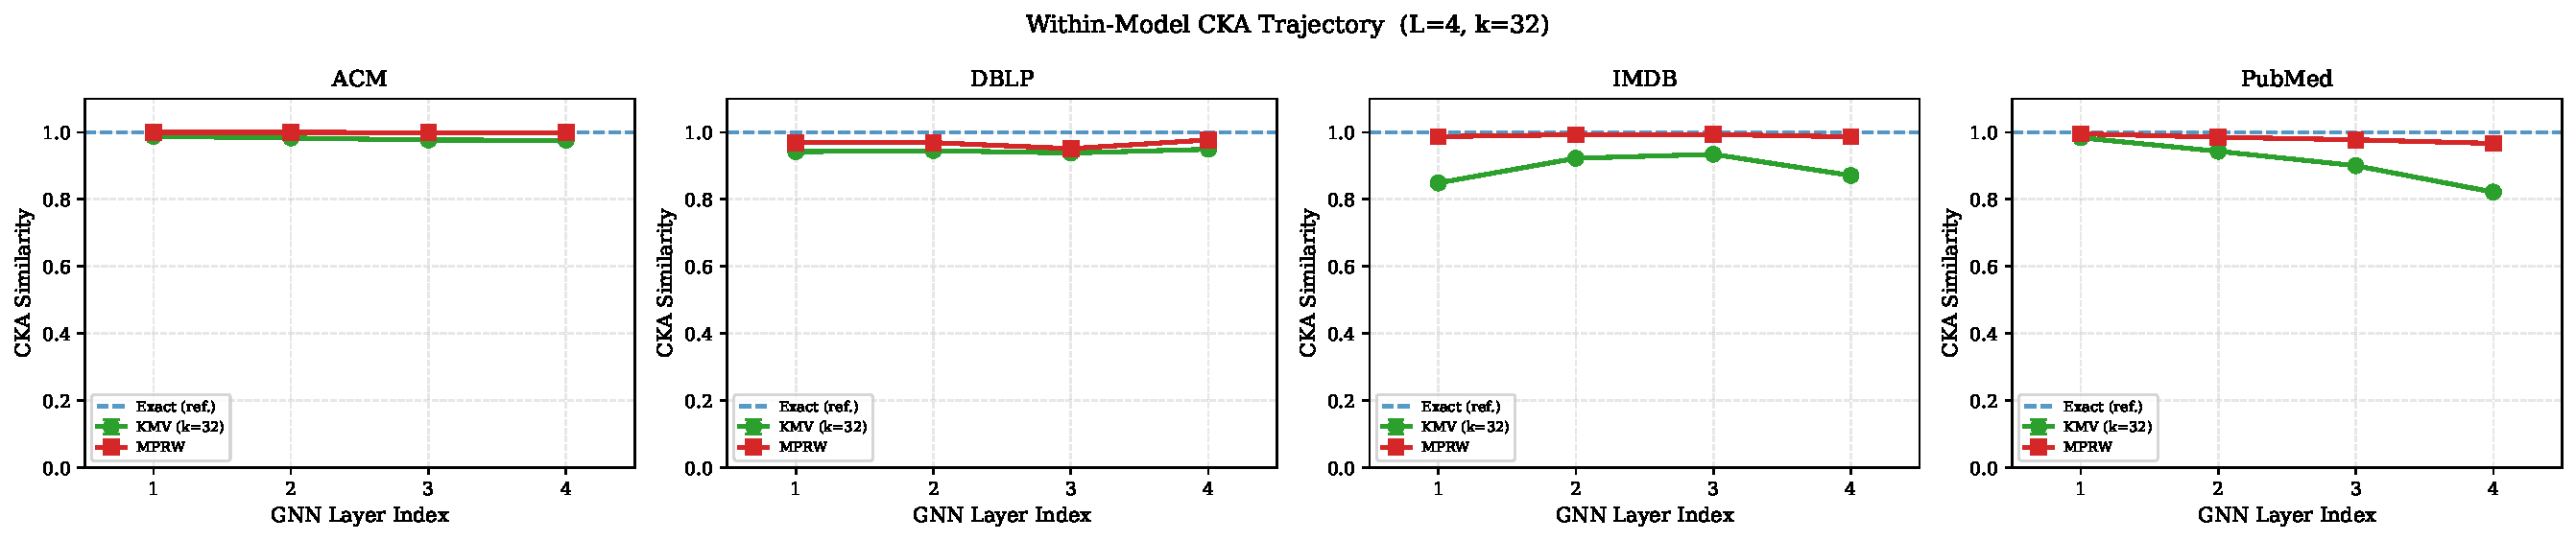
\includegraphics[width=\columnwidth]{figure/plot_cka_per_layer.pdf}
  \caption{Layer-wise CKA trajectory within a depth-4 model ($k{=}32$). Each point $\ell$ shows CKA between Exact and approximate model at intermediate layer $\ell$.}
  \label{fig:cka-layers}
\end{figure}

Figure~\ref{fig:cka-layers} shows how representational alignment evolves within a depth-4 model.
MPRW remains nearly flat near 1.0 across all layers.
KMV shows a steeper decline, consistent with the recursive drift expansion in Theorem~\ref{thm:drift}.
The degradation is \emph{bounded and predictable}: it follows the analytical decay curve rather than collapsing unpredictably.

\subsection{Large-Scale Scalability}

\begin{table}[t]
\caption{Scalability on OGB~MAG (subsets by paper count). Exact materialization times out at 60\%+ scale.}
\label{tab:scalability}
\centering\small
\begin{tabular}{lrrrrr}
\toprule
Frac. & Papers & $|E_\text{exact}|$ & Exact (s) & KMV (s) & CKA \\
\midrule
20\% & 151K & 40.4M & 30.0 & 2.58 & 0.901 \\
40\% & 319K & 263M  & 180.0 & 5.61 & 0.858 \\
60\% & --- & --- & $>$1800 & --- & --- \\
\bottomrule
\end{tabular}
\end{table}

Table~\ref{tab:scalability} demonstrates scalability on OGB~MAG~\cite{hu2020ogb}.
At 20\% scale, KMV is $11.6\times$ faster than Exact.
At 40\% scale, exact edge count grows $6.5\times$ (super-linear in $|V|$), while KMV scales linearly.
At 60\%+, Exact exceeds the 1800\,s timeout --- the $O(|V|^2)$ space/time bottleneck becomes intractable.
KMV's $O(|V| \cdot k)$ bound ensures completion at any fraction.

%% ======================================================================
\section{Discussion: KMV vs MPRW}
\label{sec:discussion}

The experimental evidence shows that KMV and MPRW deliver \emph{comparable} downstream quality.
Neither method dominates across all datasets: KMV leads on DBLP APTPA ($L{=}4$, starved budget), MPRW leads on ACM ($L{=}2$, hub-dense citations), and the two tie on IMDB and PubMed.

The selling point of KMV is \textbf{not} that it beats MPRW on quality --- it does not.
Rather, KMV offers operational advantages as a cheap, deterministic approximation of Exact:

\begin{itemize}
\item \textbf{Space}: $O(|V| \cdot k)$ vs Exact's $O(|V|^2)$.
\item \textbf{Density control}: One analytical knob $k$ --- no sweep, no calibration.
\item \textbf{Determinism}: Same sketch every run; no seed variance budget.
\item \textbf{Formal guarantees}: Finite-sample bounds (Lemma~\ref{lem:spatial}, Theorem~\ref{thm:drift}) vs MPRW's asymptotic convergence.
\end{itemize}

MPRW's higher CKA ($0.973$--$0.996$ vs $0.848$--$0.977$) reflects its importance-sampled walk structure preserving the hub geometry of the exact graph.
However, this alignment is concentrated in a class-agnostic hub subspace: higher CKA does not translate to higher F1 in 3/4 datasets.

\begin{table}[t]
\caption{KMV vs MPRW: operational comparison.}
\label{tab:comparison}
\centering\small
\begin{tabular}{lll}
\toprule
Property & KMV & MPRW \\
\midrule
Sampling      & Uniform (hash)       & Importance (walks) \\
Density ctrl  & Analytical ($k$)     & Emergent ($w$) \\
Passes        & 1 deterministic      & $w$ per node \\
Bias          & Dataset-agnostic     & Hub-biased \\
Guarantees    & Finite-sample ($k$)  & Asymptotic ($w{\to}\infty$) \\
\bottomrule
\end{tabular}
\end{table}

%% ======================================================================
\section{Conclusion}
\label{sec:conclusion}

We have shown that KMV sketch propagation---a framework originally designed for approximate hub-query centrality---can serve as a dual-purpose sketch engine: the same data structure that estimates node centrality also reconstructs graph topology for HGNN inference.
The reconstruction algorithm (Algorithm~\ref{alg:reconstruction}) operates in $O(|V| \cdot k)$ time and space, converting the $O(|V|^2)$ materialization bottleneck into a tractable linear operation.
The Spatial Variance Bound (Lemma~\ref{lem:spatial}) and Bounded Representation Drift (Theorem~\ref{thm:drift}) provide formal, computable guarantees on approximation quality that decay with sketch budget $k$ and grow predictably with network depth $L$.

Empirically, KMV achieves CKA $>0.85$ and Macro-F1 within one standard deviation of Exact on 3/4 benchmark datasets, at $3$--$4\times$ less memory and $29$--$64\times$ faster materialization.
On OGB~MAG, where exact materialization fails at 60\% scale, KMV completes in seconds.

\textbf{Future work} includes sketch-aware training (incorporating KMV stochastic edge-dropping into the training loop via variance reduction), streaming/temporal graph updates (KMV propagation is incremental), and architecture-specific drift bounds for attention-based HGNNs where $L_\sigma$ and $\|W\|_2$ have known structure.

%% ======================================================================
\bibliographystyle{ACM-Reference-Format}
\bibliography{references}

\end{document}
